\section{API design}
\label{section:APIDesign}
    The Archive service must expose its web APIs to its client so that an interaction between the application can occur.
    The Representational State Transfer (REST) \cite[Chapter.~5]{REST} architectural approach is chosen for this thesis
    to design its API. This approach is a 
    common approach to build a distributed system as it is independent of any system. Therefore using this architecture the system can later 
    evolve for any kind of system which could be used in the future providing a broader layer of flexibility to the Archive service. 
    Also, the standardized aspects of RESTful service enables a software to create a reusable elements \cite{RESTThesis}. A combination of HTTP with REST to carry out
    CRUD operations is more preferred since HTTP is widely supported by most clients and programming languages (e.g. web browsers).
    The CRUD over HTTP consists of few uniform noun based interaction that can be executed by the client \cite[p.~13]{RESTThesis}. The
    HTTP CRUD operations which are going to be implemented are described in Table \ref{table:curdHttp}.

    \begin{table}[h!]
        \centering
        \begin{tabular}{|p{2cm}|p{4cm}|p{7cm}|}
            \hline
                \textbf{HTTP Verb}  & \textbf{Description} & \textbf{Application}\\
            \hline
                POST & 
                Creates a new resources and dependent resources.
                & The POST request will be used to archive and retrieve the projects because new resources are being created for these requests.\\
            \hline
                GET & Reads the resource. & The GET request will be used to check the status of the archive and retrieve process. \\
            \hline
            PUT & Updates the resource. & The PUT request will be used to check the status of the archive and retrieve process. \\
            \hline
                DELETE & Deletes the resource. & The DELETE request will be used to delete a running archive or retrieve process. \\                
            \hline
        \end{tabular}
        \caption{CRUD interaction over HTTP in Archive service}
        \label{table:curdHttp}     
    \end{table}   
    
    Table \ref{table:archiveEndpoints} describes the API endpoint for archive, retrieve, and job status with brief description.
    \begin{table}[H]
        \centering
        \begin{tabular}{|p{6cm}|p{8cm}|}
            \hline
                \textbf{API Endpoint}&\textbf{Description}\\
            \hline
                archive/archiveProject/{{projectId}} & Archives a project given id. This is an HTTP POST method.\\
            \hline
                retrieve/retrieveProject/{{projectId}} & Restores a project given an id. This is an HTTP POST method.\\
            \hline
                job/status/{{projectId}} & Gets the status of the archive or retrieve process, given an project id. This is an HTTP GET method.\\
            \hline
                job/status/{{jobId}} & Gets the status of the archive or retrieve process, given an job id. This is an HTTP GET method.\\
            \hline
                delete/project/{{projectId}} & Deletes the archived project from the synology drive, given an job id. This is an HTTP DELETE method.\\
            \hline
        \end{tabular}
        \caption{API Endpoints description for Archive service}
        \label{table:archiveEndpoints}     
    \end{table}  
    \begin{figure}[H]
        \centering 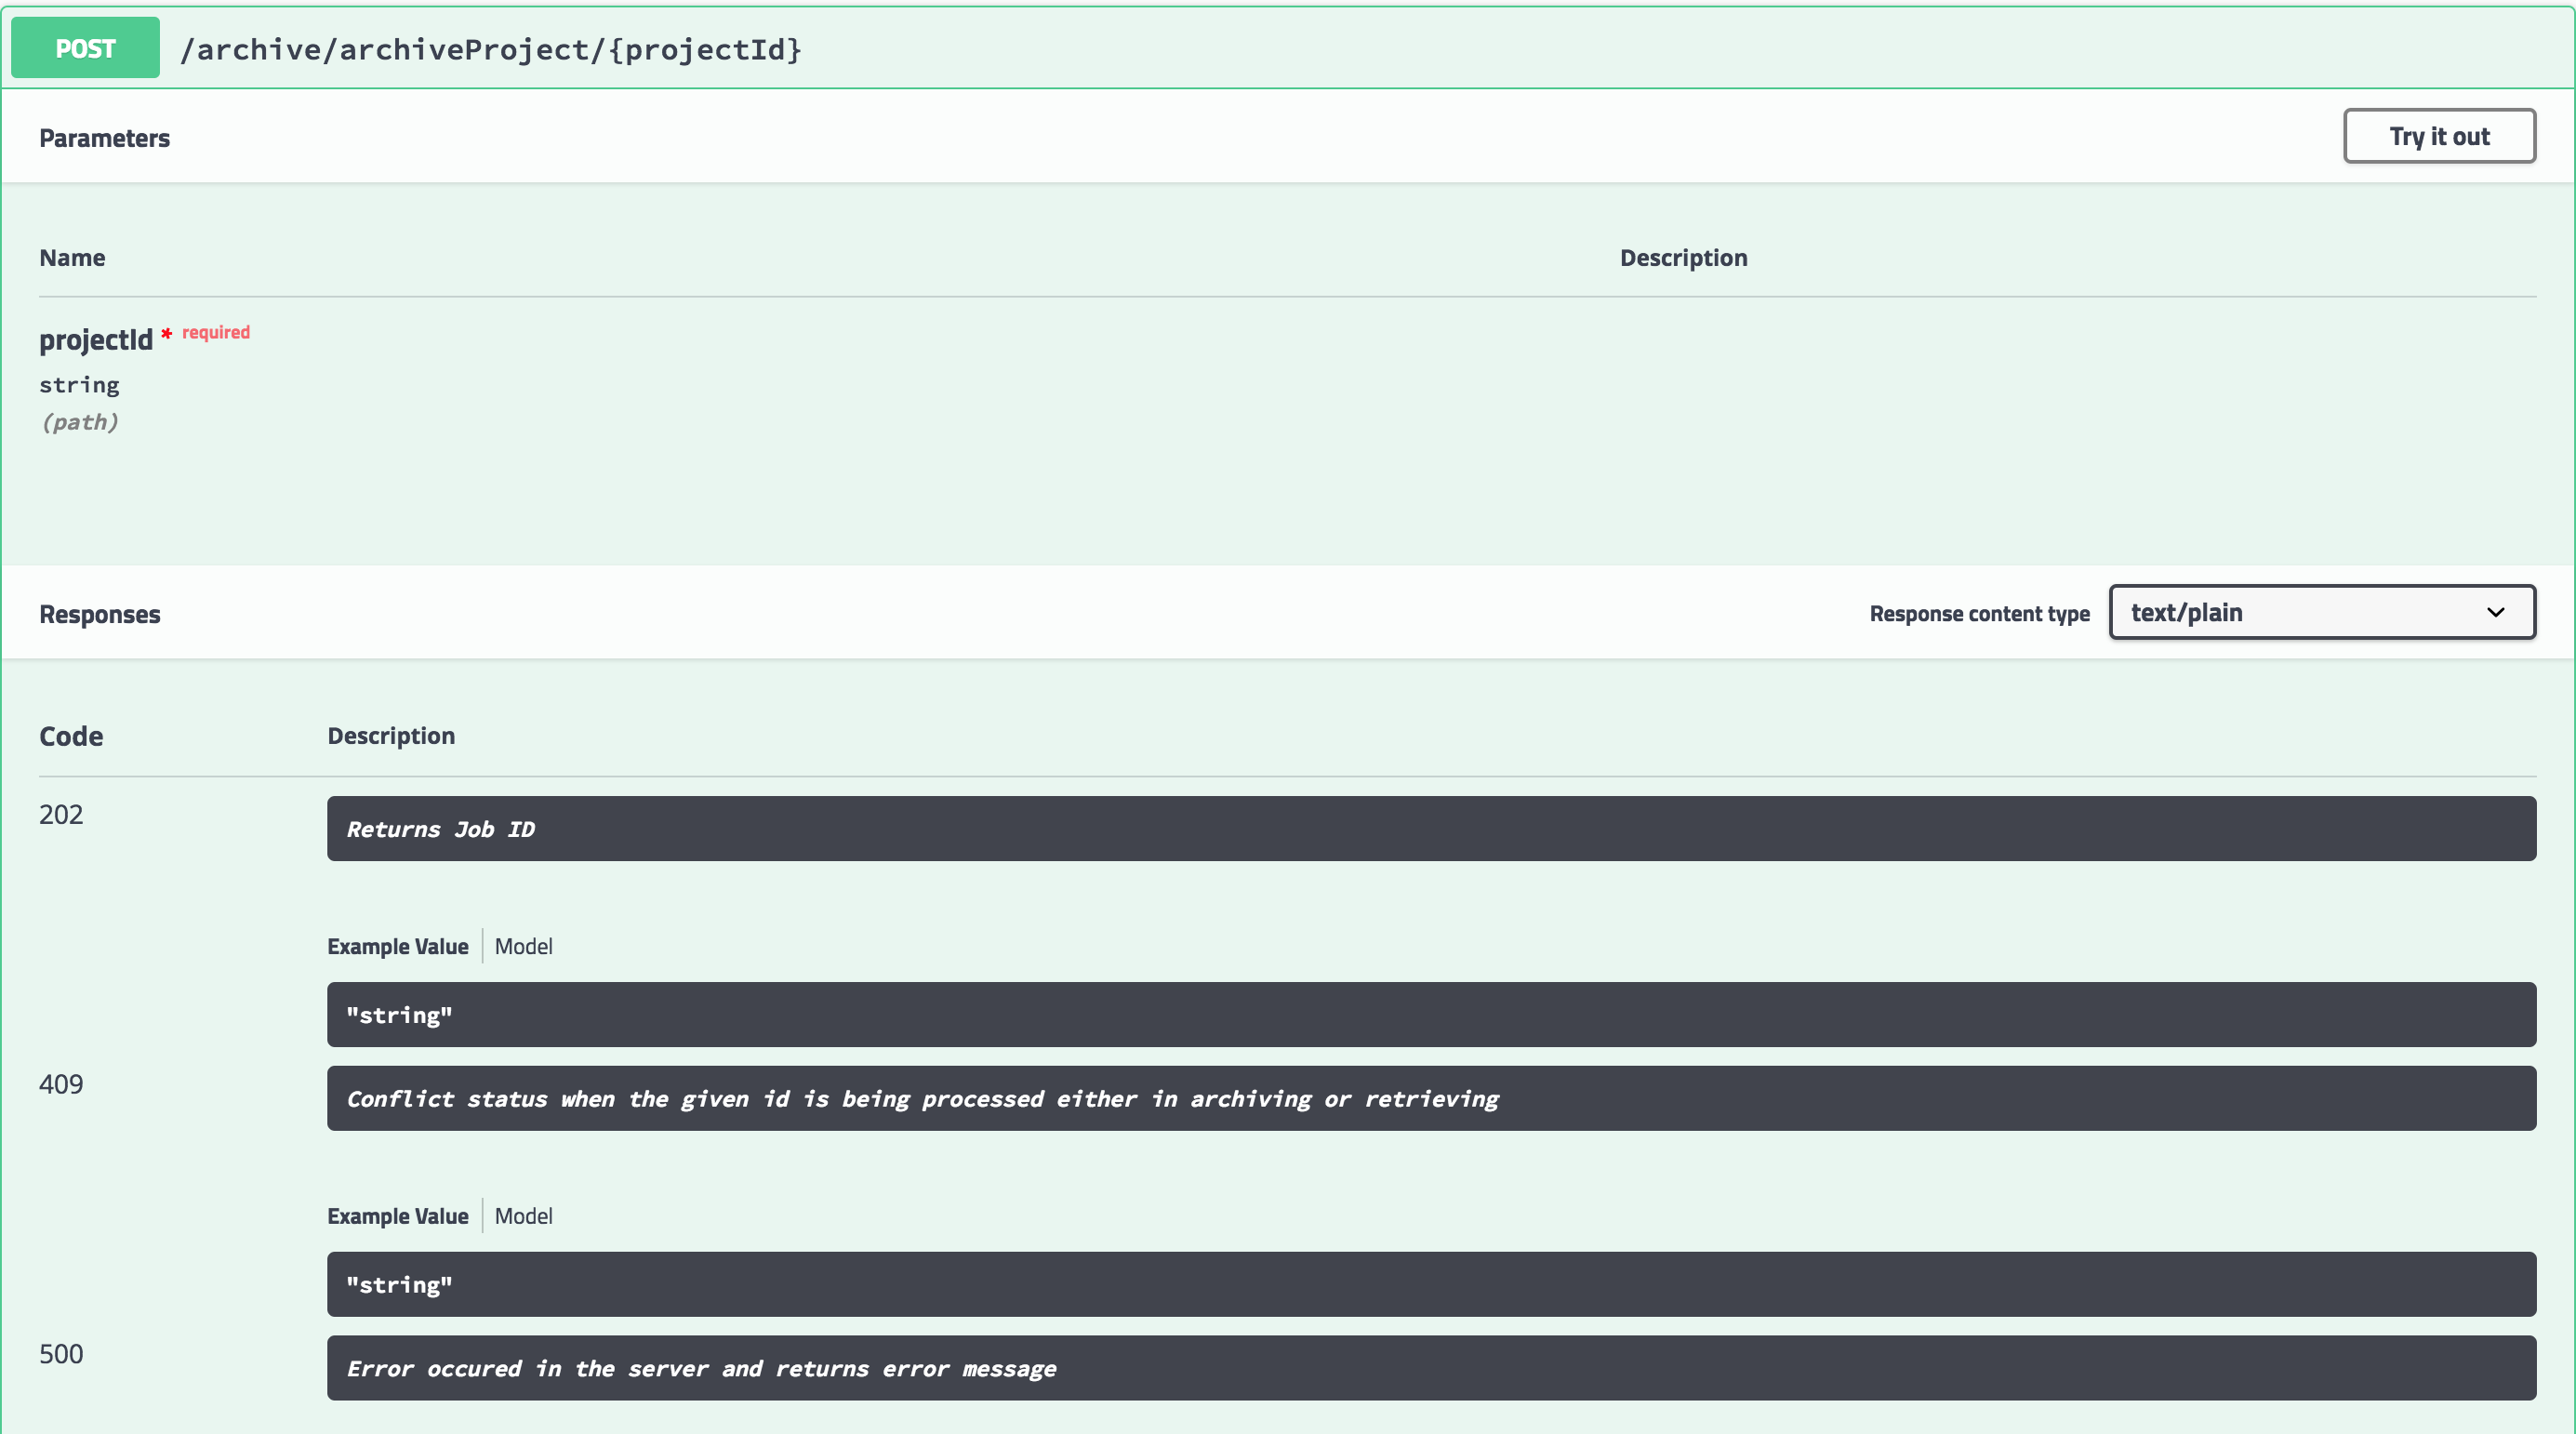
\includegraphics[scale=0.3]{grafiken/archiveSwagger.png}
        \caption{Archive endpoint shown in a swagger interface}
        \label{fig:archiveSwagger}
    \end{figure}

    \begin{figure}[H]
        \centering 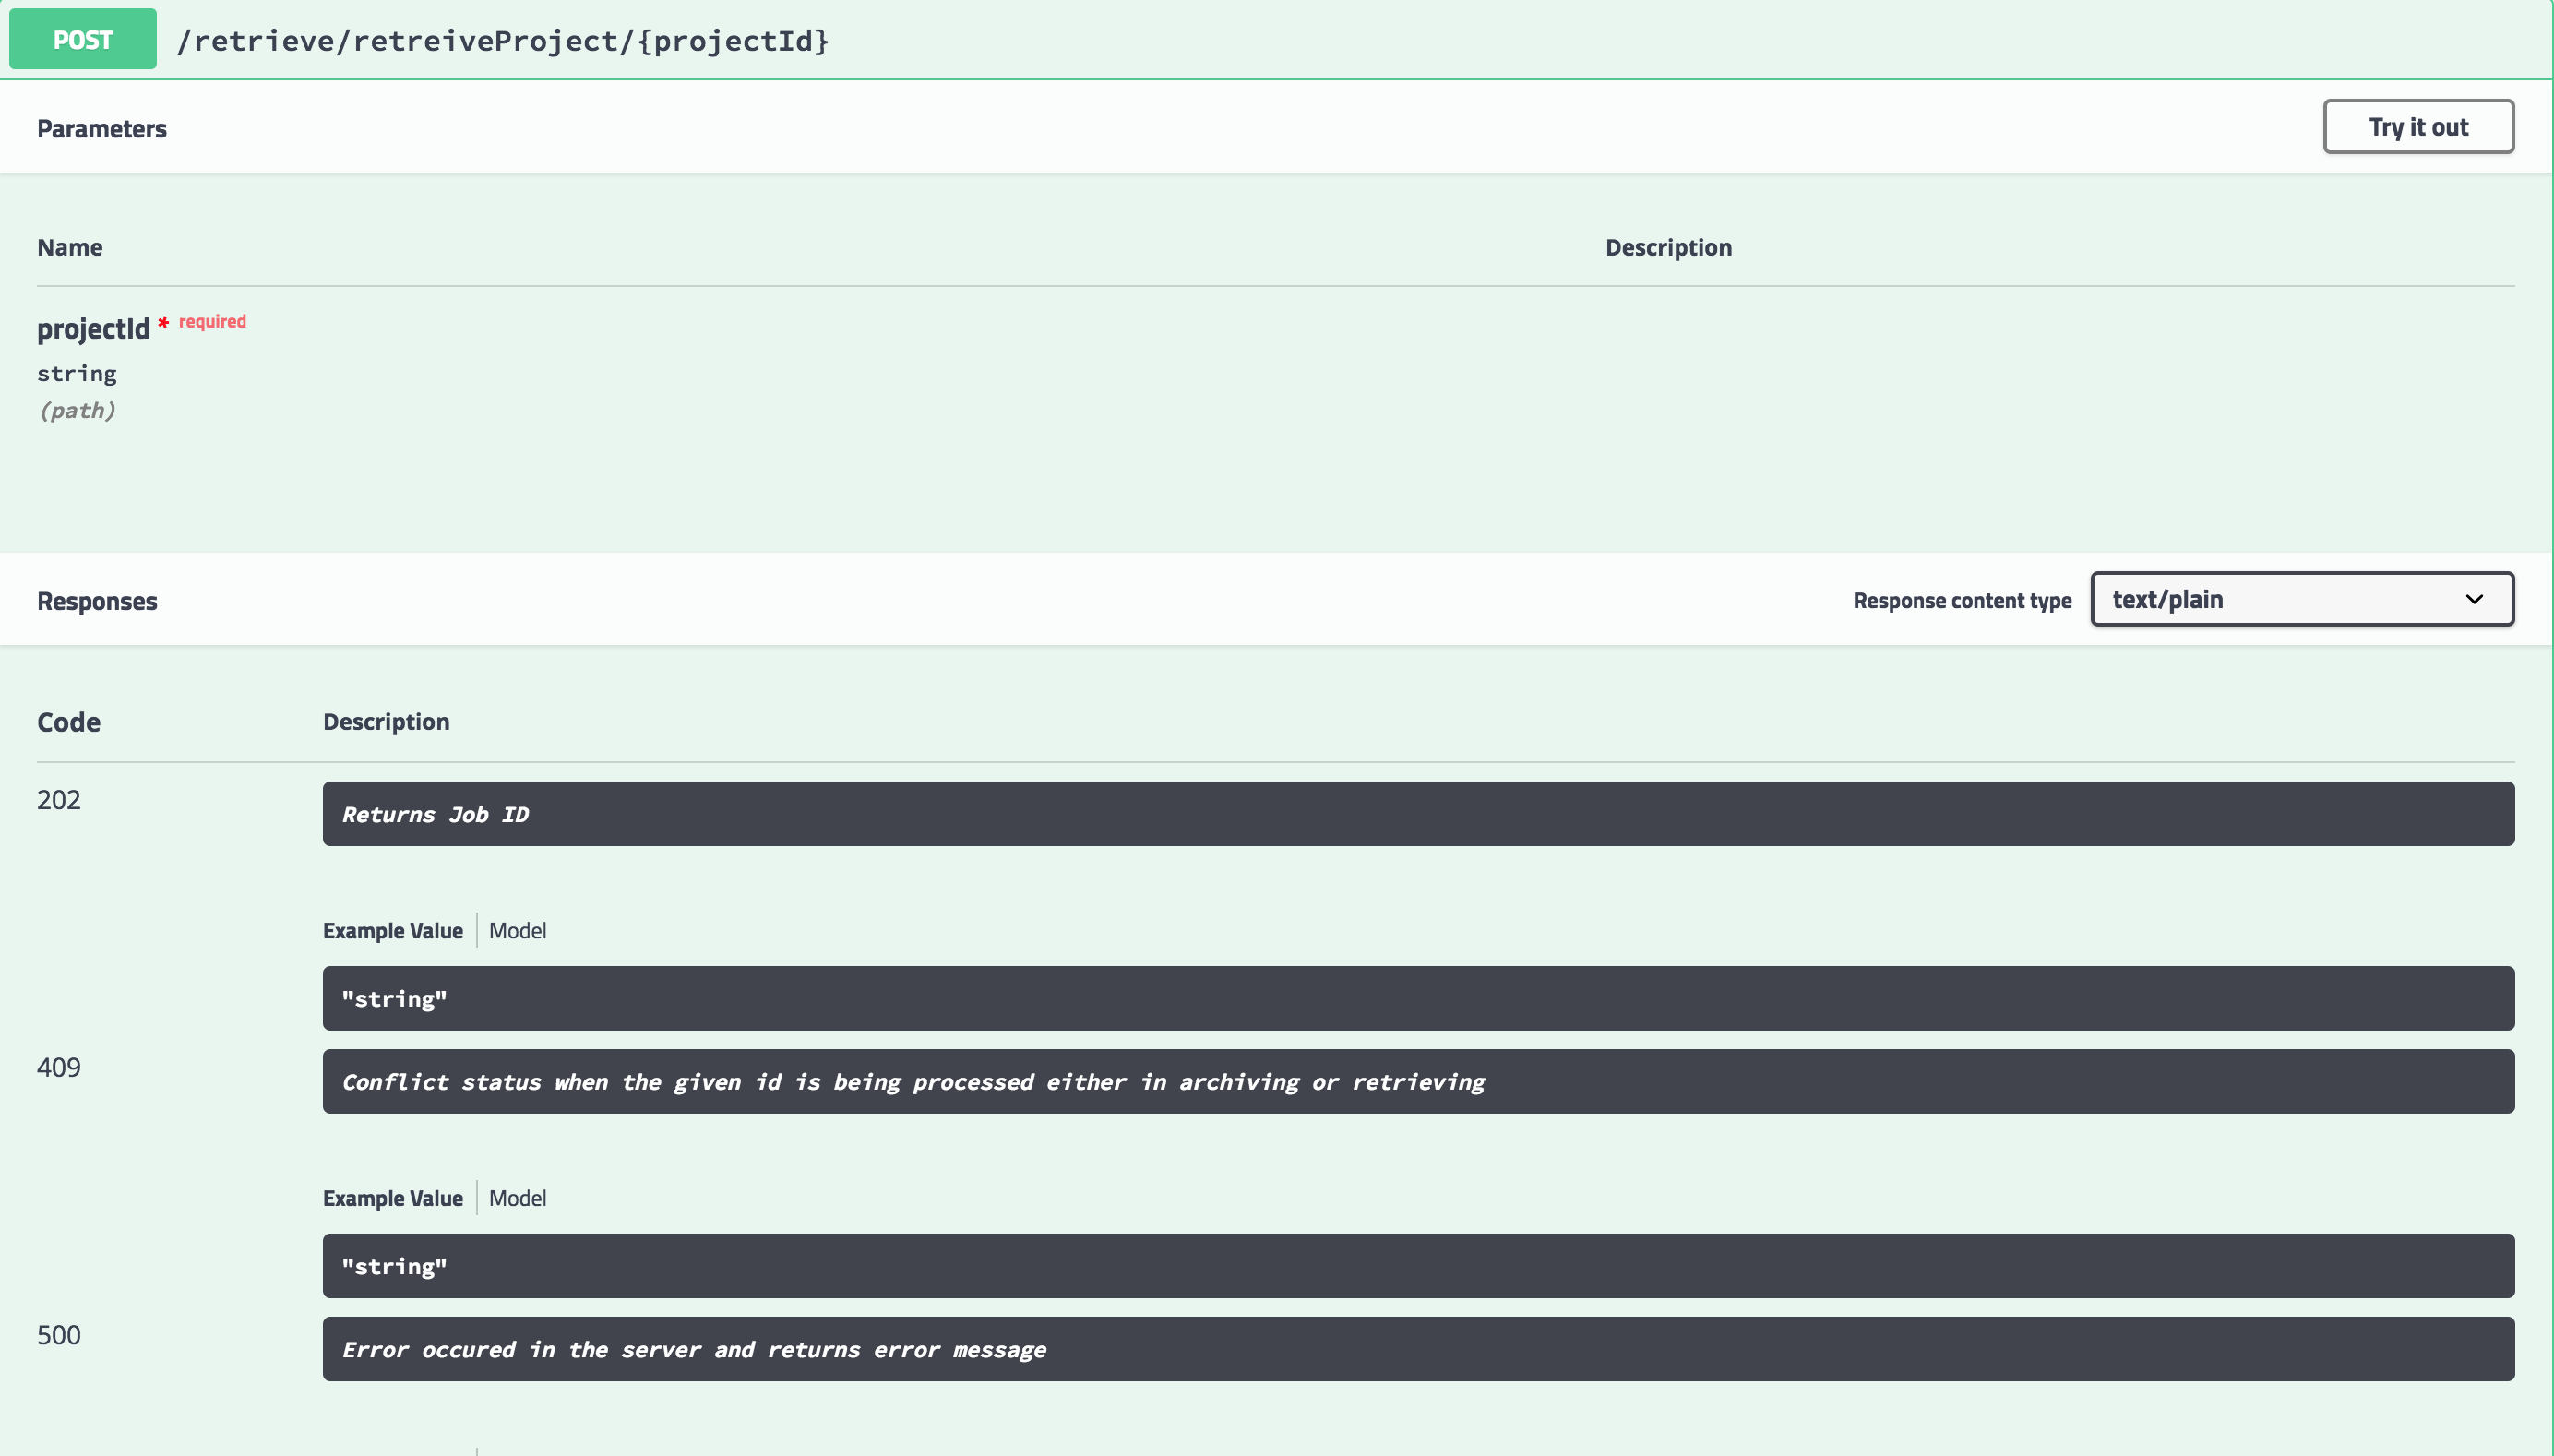
\includegraphics[scale=0.3]{grafiken/retrieveSwagger.png}
        \caption{Retrieve endpoint shown in a swagger interface}
        \label{fig:retrieveSwagger}
    \end{figure}

    \begin{figure}[H]
        \centering 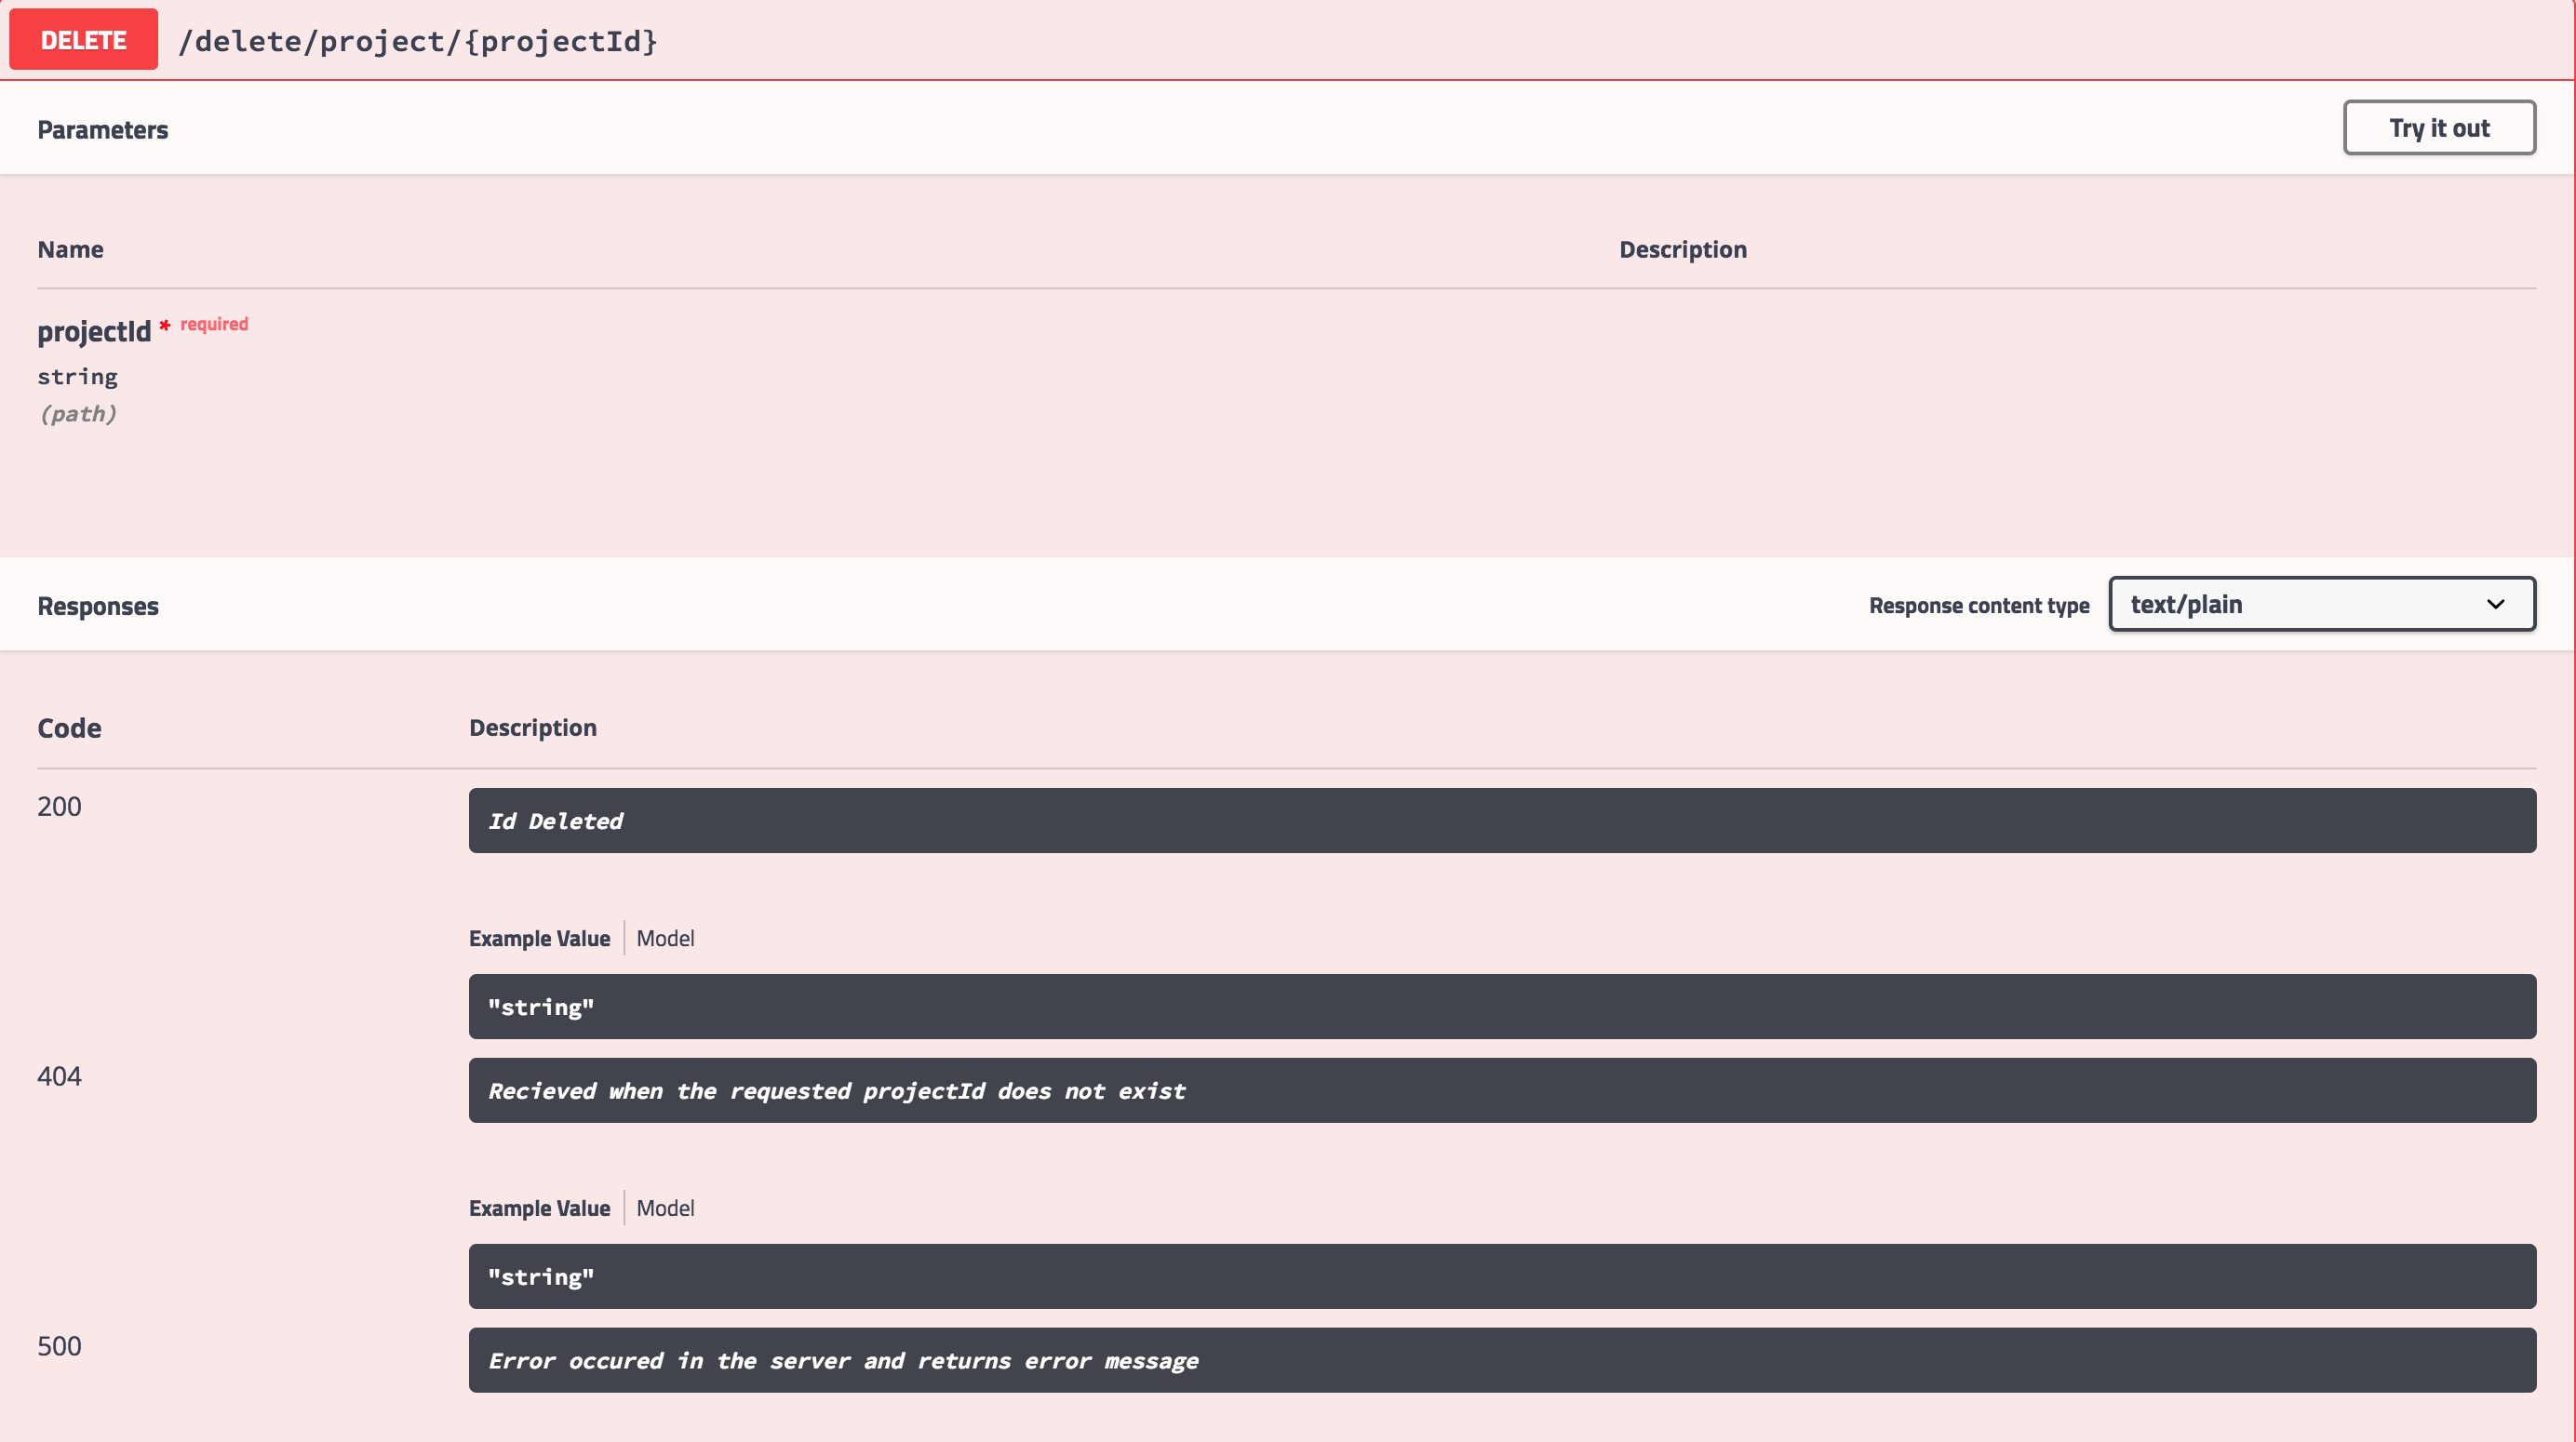
\includegraphics[scale=0.3]{grafiken/deleteSwagger.png}
        \caption{Delete endpoint shown in a swagger interface}
        \label{fig:deleteSwagger}
    \end{figure}
    
    \begin{figure}[H]
        \centering 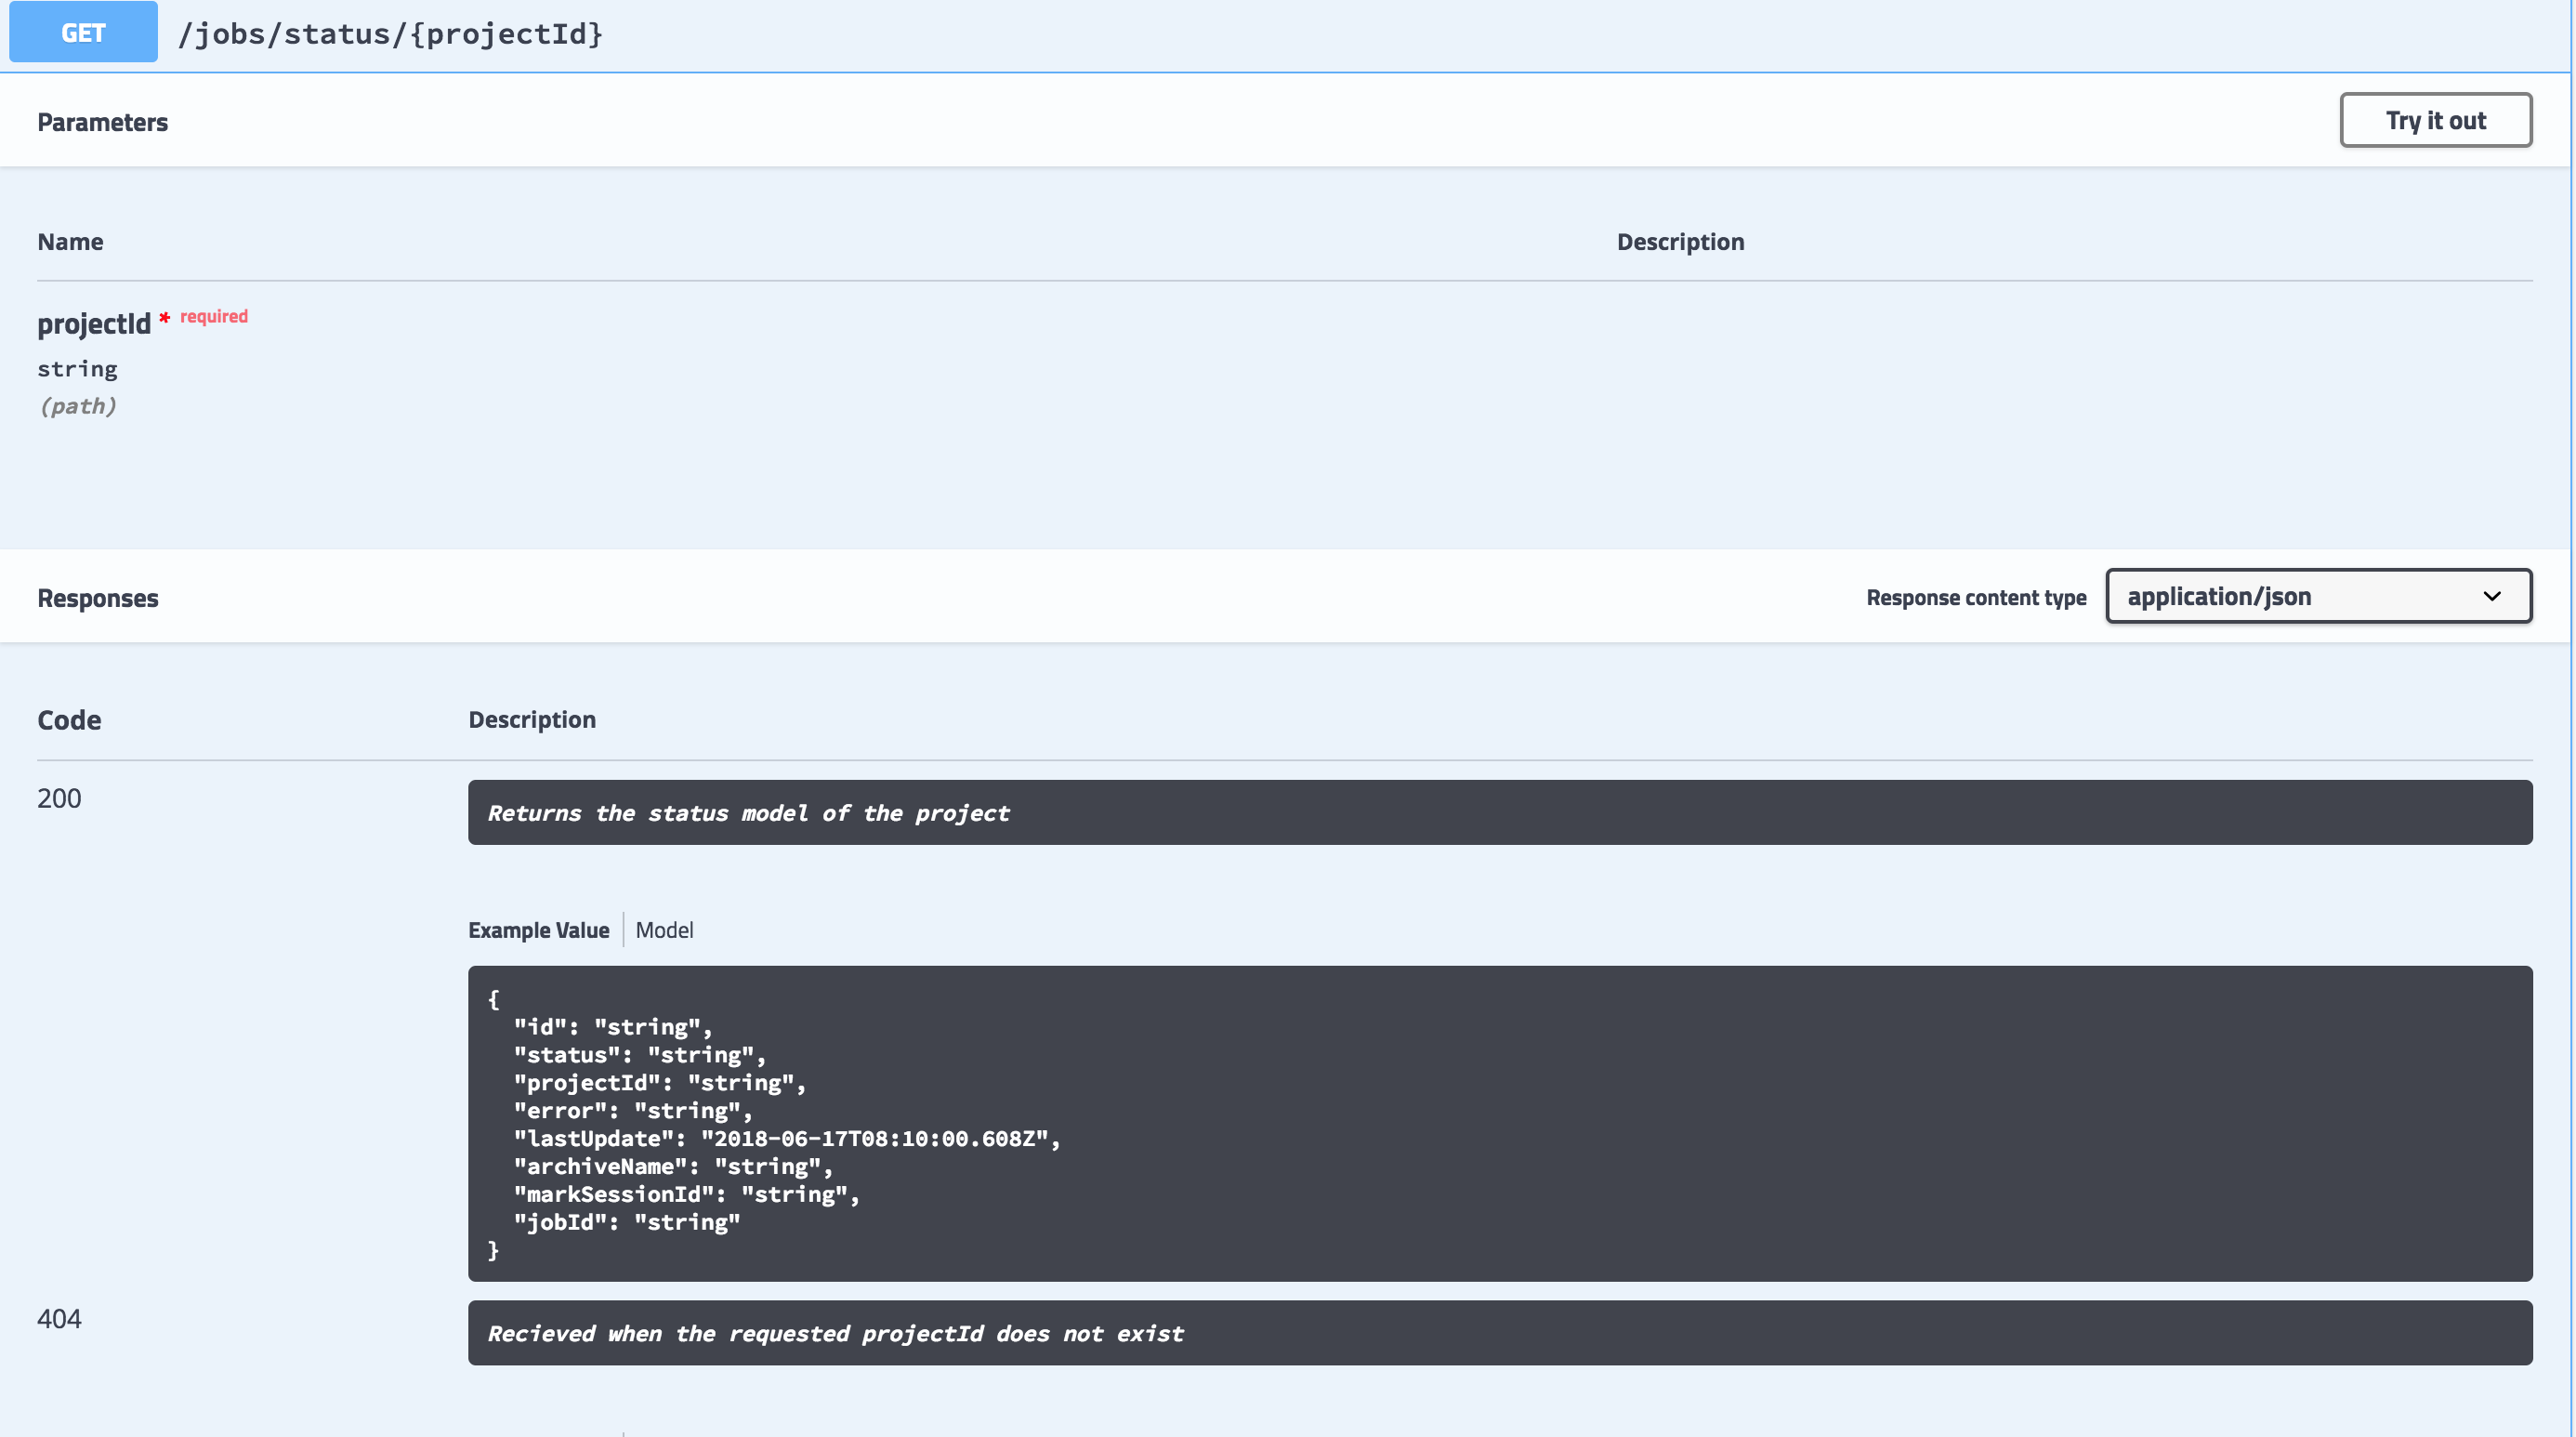
\includegraphics[scale=0.3]{grafiken/jobSwagger.png}
        \caption{Job status acknowledgment endpoint shown in a swagger interface}
        \label{fig:jobSwagger}
    \end{figure}

    Figure \ref{fig:archiveSwagger} to \ref{fig:jobSwagger} illustrates the endpoints which are going to be implemented for the Archive service. It also includes the HTTP 
    status responses the API could return depending upon the current situation i.e. 201 created when an archive process is accepted for processing by the server.
    Additionally, the API end points are designed considering the fact that more functionality could be added to the archive service without big changes needed in the client. 
    For example, the endpoint \textbf{"archive/archiveProject/{{projectId}}"} is designed thinking an archive could be also extended for other resources except the project. If later,
    the Archive service would like to support, archiving of MARS metadata resource, the endpoint would be \textbf{"archive/archiveMetadata/{{MetadataId}}"}.
    Hence, it would make it more flexible for the client to add the functionality without much effort. Also, to avoid multiple API call and
    increase the performance of the server, the get status (Figure \ref{fig:jobSwagger}) endpoint combines vital information needed for the client in one 
    request (See Listing \ref{lst:status}). 
    
\begin{lstlisting}[caption={Sucessful GET request for a archive status}, language=json,firstnumber=1, captionpos=b, label={lst:status}]
{
    "status": "PROCESSING",
    "projectId": "70C961b7-89bf-4bd5-bf61-31b6a17a15d9",
    "error": "NO ERROR",
    "lastUpdate": "2018-06-17T10:05:50.216Z",
    "archiveName": "NONE",
    "markSessionId": "AK5961b7-89bf-4bd5-bf61-31b67a15d88",
    "jobId": "855961b7-89bf-4bd5-bf61-31b6a17a15d3",
    "currentProcess": "Archive"
}
\end{lstlisting}







    
